\section{Regressão Linear}
O principal objetivo por trás da regressão linear é de estimar um valor $y \in \Re$ dado uma característica $x$.
Por exemplo, pode se estimar o valor de um estoque no dia seguinte de acordo com as vendas dos dias anteriores, os batimentos cardíacos de um atleta de acordo com a distância que percorreu, entre outras aplicações \cite{smola2008introduction}. 
 
 A Figura 1 mostra um bom exemplo de um método de regressão linear. Os pontos na figura são amostras obtidas das características $x$ da base de dados, o objetivo é criar uma função $f(x)$ que se aproxime da melhor forma dos valores observados.
\begin{figure}[H]
	\label{reg}
	\begin{centering}
		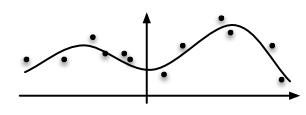
\includegraphics[width = 300pt]{img/regressao.png}
		\caption{Exemplo de regressão linear}
	\end{centering}	
	
\end{figure}
